\section{Analysis and Design}

\subsection{Requirements}

\subsubsection{Functional Requirements}
The functional architecture of DataSanitizer is categorized into seven principal requirement blocks:
\begin{enumerate}[label=\textbf{FR\arabic*.}]
  \item \textbf{Dataset Ingestion and Type Validation:} The system must accept tabular files via multipart HTTP form uploads. Permissible formats are restricted to Comma-Separated Values (\texttt{.csv}) and OpenXML Excel spreadsheets (\texttt{.xlsx}). Files exceeding 10~MB or containing zero bytes must be rejected with appropriate HTTP status codes (413 and 400). Excel files must be verified for valid ZIP container structure.
  \item \textbf{Automated Global Profiling:} Upon ingestion, the system must parse the dataset and compute comprehensive dataset-level diagnostics: total row count, column count, exact duplicate row count, sorted null-value frequency per column, sample values, and pairwise Pearson correlation coefficients ($|r| \ge 0.85$) to alert users of potential multicollinearity.
  \item \textbf{On-Demand Column Deep Profiling (Lazy Loading):} To optimize network bandwidth and server computation, detailed distribution metrics (mean, median, standard deviation, minimum, maximum, and IQR outlier count) must be computed only upon explicit user request for individual columns.
  \item \textbf{Ordered Pipeline Construction:} Users must be empowered to compose an ordered multi-step cleaning recipe containing operations such as null standardization, currency regex extraction, missing value imputation, outlier winsorization or deletion, categorical encoding, feature scaling, and feature rounding.
  \item \textbf{Dynamic Context-Aware Type Guarding:} The user interface must dynamically disable and visibly flag columns incompatible with the chosen operation (e.g., locking string/text columns when numeric operations such as StandardScaler, IQR outliers, or mean imputation are selected).
  \item \textbf{Audit Logging and Transformation Metrics:} The back-end engine must track every transformation step in an immutable audit ledger, computing initial versus final row/column counts, rows dropped, and granular descriptions of each action executed.
  \item \textbf{Processed Dataset Export:} Users must be able to download the final cleaned dataset in either standard CSV format or serialized JSON format on demand.
\end{enumerate}

\subsubsection{Non-Functional Requirements}
\begin{itemize}
  \item \textbf{Performance and Latency:} Processing and profiling of tabular datasets up to 10~MB (exceeding 20,000 rows and 30 columns) must complete in under 2.0 seconds. All pipeline transformations must be executed strictly in RAM using vectorized Pandas operations to prevent disk I/O bottlenecks.
  \item \textbf{Security and Integrity:} The server must guard against Path Traversal vulnerabilities by isolating file identifiers behind cryptographically random UUID v4 tokens. Uploaded filenames are never directly evaluated by the underlying operating system file handlers. User inputs rendered in the DOM are sanitized against Cross-Site Scripting (XSS) attacks.
  \item \textbf{Reliability and Robustness:} The application employs two-tier defensive validation: client-side pre-flight checks prevent invalid submissions, while server-side Pydantic models and algorithmic guards reject malformed requests with descriptive HTTP 400 or 422 JSON payloads without crashing the server process.
  \item \textbf{Usability and Accessibility:} The web interface must present an intuitive, single-page progressive disclosure workflow (Upload $\rightarrow$ Profile $\rightarrow$ Pipeline $\rightarrow$ Result) that guides users through complex data engineering concepts without requiring programming expertise.
\end{itemize}

\subsection{Interface Design (UI/UX)}
The DataSanitizer user interface is designed according to the principles of \emph{Progressive Disclosure} and \emph{Direct Manipulation}. The single-page application is structured into four distinct visual sections organized chronologically:
\begin{enumerate}
  \item \textbf{Step 1: Dataset Ingestion Zone:} Features a minimalist drag-and-drop file target with dynamic file selection feedback and a direct upload submission trigger.
  \item \textbf{Step 2: Exploratory Health Dashboard:} Presents high-level metric cards (Total Rows, Columns, File Identifier) alongside a real-time searchable profiling table. Columns are sorted by default in descending order of missingness, allowing users to rapidly identify polluted features. Each row includes an interactive ``View Details'' trigger that opens a focused statistical modal.
  \item \textbf{Step 3: Pipeline Builder and Real-Time Queue:} Employs a dual-column layout. The left column provides an interactive configuration panel where users select cleaning operations, adjust hyperparameters (e.g., IQR thresholds, encoding styles), and select target features. The right column renders a live, ordered execution queue displaying the exact sequence of transformations with individual deletion controls.
  \item \textbf{Step 4: Audit Summary and Export Hub:} Surfaces the final evaluation report, comparing baseline and final row/column metrics, detailing the step-by-step history ledger, and offering instant export triggers for CSV and JSON formats.
\end{enumerate}

\begin{figure}[ht]
  \centering
  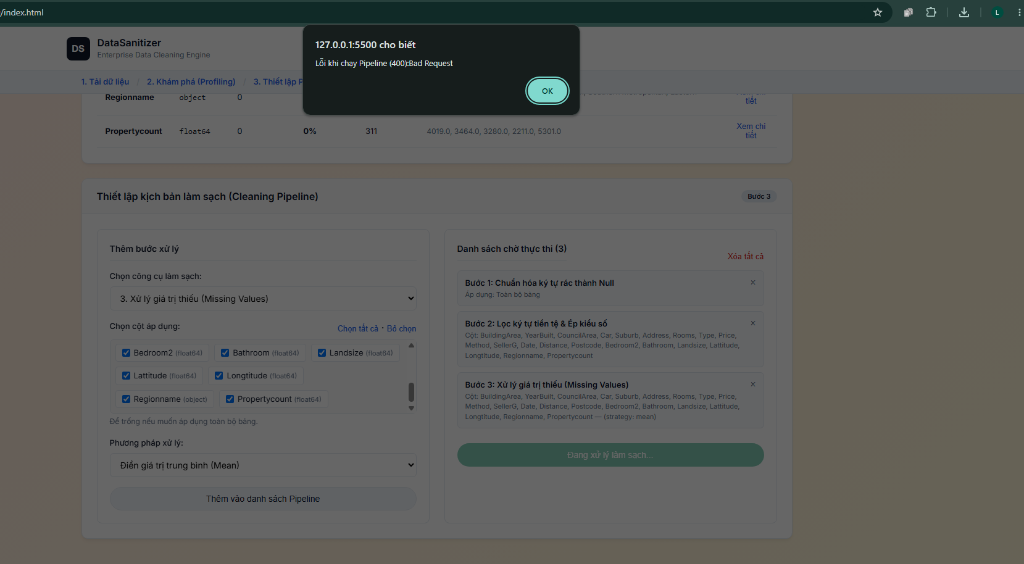
\includegraphics[width=0.92\textwidth]{figures/ui_overview.png}
  \caption{DataSanitizer interactive single-page interface showing exploratory profiling and context-aware pipeline construction on the Melbourne Housing dataset.}
  \label{fig:ui-overview}
\end{figure}

\textbf{Color Palette and Typography:}
The application employs a curated corporate palette grounded in professional data analytics aesthetics:
\begin{itemize}
  \item \textbf{Primary Brand / Structure:} Deep Slate (\texttt{\#0f172a}) and Prussian Blue (\texttt{\#1e293b}) provide authoritative contrast for navigation and typography.
  \item \textbf{Interactive Actions:} Vibrant Royal Blue (\texttt{\#2563eb}) identifies primary buttons and active indicators.
  \item \textbf{Success / Verification:} Emerald Green (\texttt{\#10b981}) signals completed transformations and safe states.
  \item \textbf{Warning / Defensive Lock:} Amber (\texttt{\#f59e0b}) and Crimson (\texttt{\#ef4444}) indicate multicollinearity risks and disabled incompatible columns.
\end{itemize}
Typography is driven by the modern sans-serif system stack (\texttt{-apple-system, Segoe UI, Roboto, Helvetica Neue}), calibrated with an 8pt baseline grid and 1.3 line-height for high numerical legibility.

\subsection{System Architecture}
DataSanitizer adopts a decoupled \textbf{Client-Server Service-Oriented Architecture (SOA)} adhering to RESTful principles \cite{fielding2000}. The architecture comprises five distinct logical tiers, as illustrated in Figure~\ref{fig:arch-flow}.

\begin{figure}[ht]
\centering
\begin{tikzpicture}[
    box/.style={rectangle, draw=PrussianBlue, fill=Solitude, thick, rounded corners=3pt, minimum width=9cm, minimum height=0.85cm, align=center, font=\sffamily\footnotesize}
]

  % Tiers with explicit vertical coordinates (no dependency on positioning library)
  \node[box] (ui) at (0, 0) {\textbf{Presentation Tier (SPA)}\\HTML5 / Modern CSS3 / Vanilla ES6 JavaScript};
  \node[box] (api) at (0, -1.45) {\textbf{API Gateway / Routing Tier}\\FastAPI Router, CORS Middleware, Pydantic Schemas};
  \node[box] (runner) at (0, -2.90) {\textbf{Pipeline Orchestration Tier}\\\texttt{pipeline\_runner.py} (Defensive Validation \& Regex Currency Parser)};
  \node[box] (engine) at (0, -4.35) {\textbf{Algorithmic Engine Tier}\\\texttt{cleaner.py} (DataCleaner) \& \texttt{profiler.py}};
  \node[box] (storage) at (0, -5.80) {\textbf{File System Cache Tier}\\\texttt{data/raw/\{file\_id\}.csv} \& \texttt{data/processed/\{file\_id\}.csv}};

  % Arrows with clear labels on the right
  \draw[->, thick, FDABlue] (ui) -- node[right, font=\tiny\sffamily, text=Astronaut] {HTTP REST / JSON Payload} (api);
  \draw[->, thick, FDABlue] (api) -- node[right, font=\tiny\sffamily, text=Astronaut] {Typed DTO / UUID Dispatch} (runner);
  \draw[->, thick, FDABlue] (runner) -- node[right, font=\tiny\sffamily, text=Astronaut] {In-Memory Pandas DataFrame} (engine);
  \draw[->, thick, FDABlue] (engine) -- node[right, font=\tiny\sffamily, text=Astronaut] {Disk Read / Write} (storage);

\end{tikzpicture}
\caption{Five-tier system architecture and end-to-end data processing flow.}
\label{fig:arch-flow}
\end{figure}

\begin{enumerate}
  \item \textbf{Presentation Tier:} Operates entirely within the user's browser, executing reactive state management, asynchronous REST communication via \texttt{fetch}, and DOM sanitization.
  \item \textbf{API Gateway / Routing Tier:} Managed by FastAPI, enforcing schema validation via Pydantic models, terminating CORS preflight requests, and dispatching tasks to background services.
  \item \textbf{Pipeline Orchestration Tier:} Intercepts pipeline arrays, validates column eligibility against real-time DataFrame dtypes, and manages regular expression currency stripping.
  \item \textbf{Algorithmic Engine Tier:} Encapsulates mathematical transformations within the vectorized \texttt{DataCleaner} and statistical profiling in \texttt{profiler.py}.
  \item \textbf{File System Cache Tier:} Persists staged raw and processed tabular files under isolated UUID paths in \texttt{data/raw/} and \texttt{data/processed/}.
\end{enumerate}

\subsection{Data Storage and Lifecycle Management}
Rather than imposing the overhead of an external relational database management system (RDBMS) for ad-hoc tabular processing, DataSanitizer utilizes a high-efficiency \textbf{Stateless File System Cache}:
\begin{itemize}
  \item \textbf{Raw Dataset Staging:} Uploaded files are immediately assigned a version-4 Universally Unique Identifier (UUID) and written directly to \texttt{data/raw/\{file\_id\}.csv} (or \texttt{.xlsx}). This guarantees constant-time $O(1)$ random access by identifier while completely eliminating filename collisions.
  \item \textbf{In-Memory State Manipulation:} During pipeline execution, the dataset is loaded into system RAM as a Pandas \texttt{DataFrame}. Transformations are applied in-place or sequentially across array pointers, avoiding repetitive, slow disk write cycles.
  \item \textbf{Processed Dataset Cache:} Upon successful pipeline completion, the clean DataFrame is serialized to \texttt{data/processed/\{file\_id\}.csv}, ready for instantaneous streaming via the download endpoints.
\end{itemize}

\subsection{API Design}
The DataSanitizer API strictly adheres to RESTful resource-oriented conventions, utilizing standard HTTP verbs, path variables, query parameters, and standardized status codes (200, 400, 404, 413, 422, 500). Table~\ref{tab:api} details the core endpoints.

\begin{table}[ht]
\centering\small
\renewcommand{\arraystretch}{1.2}
\begin{tabular}{@{}llp{5.8cm}c@{}}
\toprule
\textbf{Method} & \textbf{Endpoint} & \textbf{Functional Purpose} & \textbf{Success Code}\\
\midrule
\texttt{POST} & \texttt{/api/upload} & Ingests file multipart; verifies size and extension; returns assigned \texttt{file\_id}. & 200 OK\\
\texttt{GET}  & \texttt{/api/profile/\{file\_id\}} & Computes full dataset health profile, duplicate rows, missingness, and high correlations. & 200 OK\\
\texttt{GET}  & \texttt{/api/profile/\{file\_id\}/\{col\}} & Lazy-loads deep statistical distribution and IQR outlier count for a single column. & 200 OK\\
\texttt{POST} & \texttt{/api/clean} & Accepts ordered pipeline recipe; applies transformations; returns audit summary ledger. & 200 OK\\
\texttt{GET}  & \texttt{/api/download/\{file\_id\}} & Streams processed dataset as attachment in requested format (\texttt{?file\_format=csv|json}). & 200 OK\\
\bottomrule
\end{tabular}
\caption{Formal RESTful API contract specifications.}
\label{tab:api}
\end{table}
